\documentclass[journal,10pt,twocolumn]{article}
\usepackage{graphicx}
\usepackage[margin=0.5in]{geometry}
\usepackage[cmex10]{amsmath}
\usepackage{array}
\usepackage{booktabs}
\usepackage{mathtools}
\title{\textbf{Optimization Assignment - 2}}
\author{Chirag Shah}
\date{September 2022}


\providecommand{\norm}[1]{\left\lVert#1\right\rVert}
\providecommand{\abs}[1]{\left\vert#1\right\vert}
\let\vec\mathbf
\newcommand{\myvec}[1]{\ensuremath{\begin{pmatrix}#1\end{pmatrix}}}
\newcommand{\mydet}[1]{\ensuremath{\begin{vmatrix}#1\end{vmatrix}}}
\providecommand{\brak}[1]{\ensuremath{\left(#1\right)}}
\providecommand{\lbrak}[1]{\ensuremath{\left(#1\right.}}
\providecommand{\rbrak}[1]{\ensuremath{\left.#1\right)}}
\providecommand{\sbrak}[1]{\ensuremath{{}\left[#1\right]}}

\begin{document}

\maketitle
\paragraph{\textit{Problem Statement} - A tank with rectangular base and rectangular sides, open at the top is to be constructed so that its depth is 2 m and volume is $8 m^3$. If building of tank costs Rs 70 per sq metres for the base and Rs 45 per square metre for sides. What is the cost of least expensive tank?}

\section*{\large Solution}
\subsection*{\normalsize Theoretical approximation}
Let $l$,$b$ and $h$ are the length,width and hight of tank \\
Let $R_b$ be the base cost and $R_s$ be the sides cost.\\\ \vspace{2mm}

\section*{\large Given}
\begin{align}
h=2 &, V=8
\end{align}
\begin{align}
	V = lbh
\end{align}
where
\begin{align}
	8=2l\\
	lb=4
\end{align}
So,
\begin{align}
	b=\frac{4}{l},\hspace{1mm} & l=\frac{4}{b}
\end{align}
Total least cost is given by,\\ \vspace{1mm}
\begin{align}
    S(l)=280+180\brak{l+\frac{4}{l}}
\end{align}
\begin{align}
	S'(l)=180\brak{1-\frac{4}{l^2}}\\
        S''(l)= 180\brak{\frac{8}{l^3}} > 0
\end{align}
Thus, S($l$) has a minimum which can be obtained from (7) as \\

\begin{align}
    180\brak{1-\frac{4}{l^2}}=0\\
    \implies l^2-4=0\\
    \implies l=2
\end{align}
Substituting $l$ in equation in (6) we will get the total minimum cost and its verified 
\begin{align}
	\boxed{C_{min} = 1000}\\
	\boxed{l = 2}
\end{align}

\subsection*{\normalsize Gradient descent}
Let $l$ be the length of tank \\ \vspace{1mm}
The Total least cost of tank is expressed as
\begin{align}
	\label{eq:vol_varx}
	f(l) = 280 + 180\brak{l+\frac{4}{l}}
\end{align}
Using gradient ascent method we can find its minima\\ \vspace{2mm}

    \begin{align}
        x_{n+1} &= x_n + \alpha \nabla f(x_n) \\
        \implies x_{n+1} &= x_n + \alpha \brak{180\brak{1-\frac{4}{l^2}}}
    \end{align}
    
Taking $x_0=2,\alpha=0.001$ and precision = 0.00000001, values obtained using python are:
    
    \begin{align}
        \boxed{\text{Minima} = 1000}\\
        \boxed{\text{Minima Point} = 2}
    \end{align}

\begin{figure}[t]
	\centering
	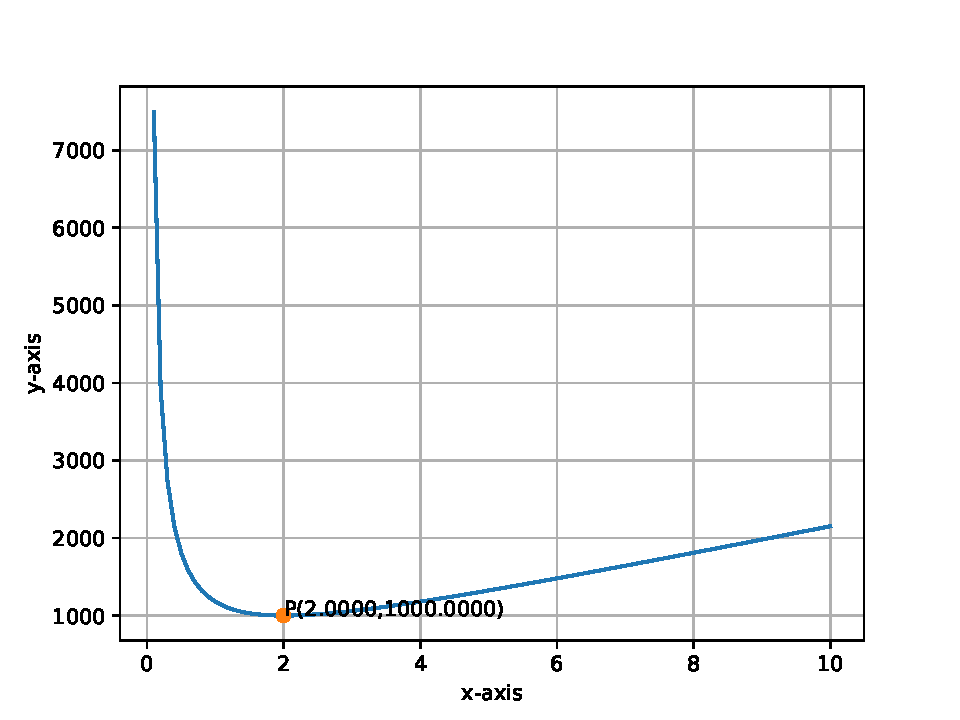
\includegraphics[width=1\columnwidth]{opt.pdf}
	\caption{Graph of $S(l)$ vs $l$}
	\label{fig:graph_fx}
\end{figure}

\end{document}